\documentclass[12pt,a4paper,twoside]{report}

\usepackage{comment}
\usepackage{listings}
\usepackage{xcolor}
\usepackage[T1]{fontenc}
\usepackage{listingsutf8}

\usepackage[T1]{fontenc}
\usepackage[utf8]{inputenc}
\usepackage{lmodern}
\usepackage{microtype}

\usepackage[a4paper,margin=1in]{geometry}

\usepackage{xcolor}
\usepackage{graphicx}
\usepackage{capt-of}
\usepackage{float}
\usepackage{tikz}

\usepackage{array}
\usepackage{booktabs}
\usepackage{multirow}
\usepackage{tabularx}
\usepackage{longtable}

\usepackage{fancyhdr}
\usepackage{lastpage}

\usepackage{amssymb}
\usepackage{amsmath}

\usepackage[labelfont=bf,font=small]{caption}


\usepackage{enumitem}
\setlist{nosep}


\usepackage{pdfpages}

\usepackage{titlesec}
\titleformat{\chapter}[hang]
  {\normalfont\huge\bfseries}
  {\chaptertitlename\ \thechapter\ --}
  {0.5em}
  {}

\usepackage{setspace}
\onehalfspacing

\usepackage{enumitem}
\setlist[enumerate]{label=(\arabic*)}

\usepackage{csquotes}
\usepackage[style=ieee,backend=bibtex]{biblatex}
\addbibresource{references.bib}

\definecolor{linkblue}{HTML}{145680}
\definecolor{headergray}{gray}{0.35}

\usepackage{hyperref}
\hypersetup{
    colorlinks=true,
    linkcolor=linkblue,
    urlcolor=linkblue,
    citecolor=linkblue,
    pdfnewwindow=true
}

\pagestyle{fancy}
\fancyhf{}

\fancyhead[LE]{\color{headergray}\sffamily\bfseries Essence C - A new programming language}
\fancyhead[RO]{\color{headergray}\sffamily\bfseries\nouppercase{\leftmark}}

\fancyfoot[C]{\sffamily Page \thepage\ of \pageref*{LastPage}}

\renewcommand{\chaptermark}[1]{\markboth{\chaptertitlename\ \thechapter\ -- #1}{}}

\fancypagestyle{plain}{\pagestyle{fancy}}

\renewcommand{\headrulewidth}{0pt}
\setlength{\headheight}{24pt}
\setlength{\headsep}{32pt}

\setlength{\parskip}{0.6em}
\setlength{\parindent}{0pt}

\begin{document}

\begin{titlepage}
  \setstretch{1.125}
  \centering
  
  \begin{tikzpicture}
    \clip (0,0) circle (1cm);
    \node at (0,0) {
\includegraphics[height=2cm]{logo.png}};
    \draw[line width=2pt] (0,0) circle (1cm);
  \end{tikzpicture}\par\vspace{0.3cm}

  {\color[HTML]{8b008b}\LARGE\textbf{Essence C}\par\vspace{0.7cm}}
  
  {\large\textbf{A new programming language to advance link-time optimizations by faciliating the continuum of static and dynamic modules.}\par}
  
  \vspace{0.7cm}
  
  {\bfseries David Callanan\par}
  {\bfseries 21444104\par}
  
  \vspace{0.7cm}
  
  {Final Year Project -- 2026\par}
  {B.Sc. Single Honours in Computational Thinking\par}
  
  \vfill
  
  
\includegraphics[width=0.375\textwidth]{mu_full.png}
  
  \vfill
  
  {Department of Computer Science\par}
  {Maynooth University\par}
  {Maynooth, Co. Kildare\par}
  {Ireland\par}
  
  \vspace{1cm}
  
  {A thesis submitted in partial fulfilment of the requirements for the\par}
  {B.Sc. Single Honours in Computational Thinking.\par}
  
  \vspace{1cm}
  
  {\textbf{Supervisor: Dr. Phil Maguire}\par}
  
  \vspace{1cm}
  
\end{titlepage}

\newpage

\tableofcontents

\newpage

\thispagestyle{empty}


\section*{Declaration}
\addcontentsline{toc}{section}{Declaration}

I hereby certify that this material, which I now submit for assessment on the program of study as part of the B.Sc. Computational Thinking qualification, is entirely my own work and has not been taken from the work of others -- save and to the extent that such work has been cited and acknowledged within the text of my work.

I hereby acknowledge and accept that this thesis may be distributed to future final year students, as an example of the standard expected of final year projects.


\vspace{2cm}

Signed: \rule{5cm}{0.4pt} \hfill Date: \rule{3cm}{0.4pt}

\vspace{2cm}

\null
\newpage
\thispagestyle{empty}


\section*{Acknowledgements}
\addcontentsline{toc}{section}{Acknowledgements}

A massive thanks to Dr. Phil Maguire, friends, and peers for inflicting levels of motivation I might never reciprocate.

Some brief gratitude to Anthropic for their powerful GenAI models, though other models were preferred due to cost reasons.

\vfill
\null

\newpage

\begin{abstract}

The logic of computer software is primarily expressed using programming languages, but the balance between versatile and efficient programming languages remains a major challenge. Changes to the execution environment of a program can impact performance, or worse, cause incompatibilities that require major refactoring. Developers often maintain multiple branches of a codebase to keep performance to acceptable levels. One particular difference between execution environments is whether individual modules are statically linked at compile-time or dynamically resolved at runtime. In this research project, we propose a prototype programming language called ``Essence C'' that better supports the continuum of static and dynamic modules, by allowing the programmer to write code \textit{once}, that is agnostic to the linking strategy. This is achieved by designing unique language features that are inspired by \textit{zero-cost abstraction} principles. By taking advantage of LLVM's intermediate representation, it is possible to advance the state-of-the-art of link-time optimizations across module boundaries. The performance of these optimizations is assessed by benchmarking four simple hardware operations in a proof-of-concept operating system kernel, consisting of \textit{C}, \textit{Essence C}, \textit{NASM}, and \textit{LLVM IR}. The ability for large language models to assist with using \textit{Essence C} is also evaluated.

\end{abstract}

\newpage

\chapter{Introduction (930)}

\section{Overview}

This project is concerned with the research and development of a novel programming language, Essence C, that facilitates the continuum of static and dynamic modules in low-level software development. The prototype henceforth discussed is accomplished by designing unique language features and implementing bespoke optimizations pursuant to these features. Kernel development is used as a case study throughout the research phase and evaluation phase.

\section{Motivation}

Software development is becoming very popular, with graduates now unable to find jobs due to a massive spike in educational resources allocated to this field. With the use of LLM agents gaining traction, keeping a codebase clean may be harder than ever before. There is now serious competition in programming language design due to two reasons. Firstly, an LLM's ability to navigate a codebase effectively depends on the structure imposed directly by the language, given the reduced structural input from the programmer. Techniques that minimize duplicated effort in a codebase is expected to minimize context rot and reduce the agentic workflow bills. Secondly, agents are at risk of optimizing their development in highly trained-on environments (e.g. JavaScript, web-based, and \textit{React.js} environments), leaving less-prevalent low-level languages behind unless the agent can learn from on-the-fly tool calls. Highly structured languages with a superb type system, high cohesion of language concepts, and excellent documentation may make up for the lack of training. An effective module system alongside other novel language features has the potential to transform the way humans and agents reason about their software. This includes the desire to be able to freely architect software for organizational, abstractional and future-proofing purposes without compromising performance or compatibility. Developers are often fed up with having to rewrite code when environmental changes are bestowed upon them. This thesis focuses on one key area where such increased flexibility is desirable: linking and dispatch strategies for modules and objects alike.

\section{Methodology}

To address the objectives of this research, a design-science methodology is employed with a focus on continued interation and evaluation of ``Essence C''. This approach was selected because the project is concerned with the implementation of a novel programming language that advances the flexibility and performance of modules in software development, and thus requires a design and implementation process that is informed by ongoing evaluation.

The structure of this thesis is organized to reflect this methodology. First, Chapter 2 reviews existing literature, both theoretical and technical, focusing on how kernels optimize static calls and how the LLVM toolchain is effective for programming language development. Next, Chapter 3 summarizes the key aspects of the problem, including the functional and non-functional requirements. Then, Chapter 4 considers separately the design elements and implementation details of the solution. Penultimately, Chapter 5 evaluates the success of the project in the areas of snapshot testing, performance benchmarking, and GenAI comprehension. Finally, Chapter 6 concludes with an overall assessment, limitations, and future work.

\section{Success Criteria}

Success is evidenced by the following deliverables:

\begin{enumerate}
	\item A functional prototype compiler that implements the designed module system;
	\item Documentation of the module system and other core language features;
	\item A simple IDE extension that provides syntax highlighting to the programmer;
	\item A body of research into the continuum of static and dynamic modules in software development, with kernel development as a case study;
	\item An implementation of link-time optimization techniques that leverage the designed module system;
	\item An evaluation of the effectiveness of these optimizations through the benchmarking of a prototype operating system kernel;
	\item A monorepo containing extensive git history, demonstrating ongoing development progress;
	\item A final thesis (that you are reading) detailing the research, design, implementation and evaluation of the project.
\end{enumerate}

Some considerations will be out of scope for this project, such as the performance of compilation, the level of detail of compilation errors, and the implementation of standard library functions and advanced type system features.

\section{Use of Generative AI}

Two notable GenAI tools have been used to assist with the research and development of this project.

\begin{enumerate}

\item The first is \href{https://t3.chat}{t3.chat}, a web application that consolidates numerous large language models into a streamlined chat interface \cite{t3chat}. The user can experiment with different models to understand which models are best suited for the task at hand.
Both research and programming tasks have benefited from the use of this tool.
The tool was primarily used to steer the work in the right direction, and to identify the concepts, libraries and resources through which further research could be conducted. For transparency, all LLM prompts have been included in \textbf{Appendix C}. This appendix was generated programatically by using the JSON export facility and filtering relevant chats.

\item The second is the tab-complete feature of \href{https://github.com/features/copilot}{GitHub Copilot}. This tool has encouraged rapid development and iteration through its behaving as a glorified autocomplete. From experience, the tool's context is severely limited, forcing the developer to have genuine knowledge of the codebase and its architecture. This is beneficial for projects that require significant unique input from the developer, in contrast to rehash projects that benefit more directly from LLM assistance. The latest iteration of this feature allows completions for lines that are away from the cursor, which has been a game-changer.

\end{enumerate}

Some experimentation with GitHub Copilot agent mode was conducted, with notable issues identified. Firstly, the development speed was impeded by slow model response times, lack of funds, and internet connectivity issues. Secondly, there was a great difficulty in referencing contributions made by this tool due to (1) tool calls that modify the codebase directly and (2) significant implicit pollution of the context window as the agent navigates the respository. As such, with an exception for debugging, usage of this tool was suspended.

The logo on the cover page was generating using \textit{Nano Banana Pro}.

\chapter{Technical Background (1200)}

\section{Literature Review}

\subsection{Static vs dynamic dispatch}

There are two primary ways for methods of objects (or equivalent constructs) to dispatch calls: static dispatch or dynamic dispatch. When the exact implementation of a method is known at compile-time, static dispatch is typically favoured, involving a direct assembly call to the method. Since the method is known at compile-time, the compiler can use immediate addressing mode, which is most efficient. In contrast, when the exact implementation of a method is not decided until runtime (or if the compiler cannot prove otherwise), dynamic dispatch is required, which involves an indirect call through a vtable or similar structure.

\subsection{Static vs dynamic linking}

There is much overlap in the literature between dispatch techniques and linking techniques. Linking focuses on larger units of code, often referred to as modules or libraries, as opposed to objects. This is crucial in C where there is no inbuilt notion of static vs dynamic dispatch. Rather, C programmers often use seperate compilation units to allow the user to substitute implementations. Unfortunately, architectural limitations often result in the use of the unfavourable PIMPL idiom which can tank performance, but I digress.

To ditto the above, there are two primary ways for compilation units to be linked: static linking and dynamic linking. When the exact source code (implementation) of a module is known at compile-time, static linking is typically favoured, involving the direct inclusion of the module's code into the final executable. Then, the compiler can use immediate addressing to invoke functions or access data from this module. In contrast, when the exact source code of a module is not decided until runtime, dynamic linking is used which typically requires a Procedure Linkage Table (PLT) and Global Offset Table (GOT).

Various techniques are already employed to optimize dynamic linking:

\begin{enumerate}
  \item Some architectures use the ``relaxation'' technique to replace indirection at runtime by modifying the assembly instructions.
  \item Good compilers can perform PLT rewriting at compile-time if the nature of the calls is known.
  \item Bespoke replacement (e.g. Linux kernel static calls).
\end{enumerate} 

However, a primary concern remains: Various optimization techniques such as inlining become impossible due to this indirection.

\subsection{Module loading in the Linux kernel}

It was found that the potential inefficiencies of dynamically loaded modules were already considered by the Linux kernel developers, and boutique infrastructure was developed to partially mitigate this.

The Linux kernel benefits from their ``static\_call'' system, which uses a combination of C macros, custom compilation/linking steps, and runtime logic to patch function calls to be more efficient. Any calls that may need to be dynamically swapped at runtime can engage with the ``static\_call'' system to improve performance and automate the repetetive assembly logic. The process is summarized below.

\subsubsection{Macro system}

Each static-call function is implemented using the ``DEFINE\_STATIC\_CALL'' macro, which takes in (1) a handle name, and (2) a pointer to the initial implementation for this handle. This macro is used at the top-level. Then, the programmer can use the ``static\_call\_update'' macro at any point, taking in the same parameters, to alter the implementation for a particular handle at runtime. Alas, the programmer can use the ``static\_call'' macro to invoke the handle like a traditional function. Here is some example pseudo-code:

\begin{verbatim}
void implementation_a(int value) { ... }
void implementation_b(int value) { ... }

DEFINE_STATIC_CALL(foo, implementation_a);

void main() {
  static_call(foo)(27);
  static_call_update(foo, implementation_b);
  static_call(foo)(27);
}
\end{verbatim}

The ``static\_call'' macro also uses the inline assembly ``.pushsection'' and ``.popsection'' directives to temporarily relocate the code to a unified object section that can be picked up in the custom compilation step.

A crucial takeaway is that the lack of direct language support has forced the need for a custom macro setup. Understandably, programmers in different codebases may not be so adamant to commit resources to such a setup in the same way the Linux kernel developers have.

\subsubsection{Custom compilation step (objtool)}

The kernel needs to remember where the call sites are when the implementation is swapped at runtime. To achieve this, the kernel includes an extra build step that investigates the aforementioned object section to locate all relevant call sites. It then builds up a table that can be inspected at runtime to ensure no call sites are missed. There are many more intricacies that are not mentioned and have not been studied in too much detail.

If you explore the source code for the Linux kernel, you will come across the \href{https://github.com/torvalds/linux/blob/master/include/linux/static_call_types.h}{static\_call\_types.h} file, containing the following:

\begin{verbatim}
/*
 * The static call site table needs to be created by external tooling (objtool
 * or a compiler plugin).
 */
struct static_call_site {
	   s32 addr;
	   s32 key;
};
\end{verbatim}

\subsubsection{Trampoline solution}

The easy solution to alter the implementation of a function at runtime is to use a trampoline (an extra dynamic jump instruction that is resolved at runtime). This is slow and is merely a backup option.

Insert diagram.

\subsubsection{Inlining solution}

Great news, inlining refers to the trampoline call, not inlining the function body itself.

(Well not so great news, but at least there is more merit to this project).

\subsubsection{Spectre}

Since the infamous Spectre exploit in 20XX, 

\subsection{Inlining and IR-level linking}

\section{Technical Material}

\subsection{LLVM Intermediate Representation}

LLVM was found to be a practical compilation target for low-level programming languages due to (1) its target-independent code generation \cite{llvmcodegen} and (2) its integration capabilities with existing programming languages thanks to ABI interoperability (including some recent improvements \cite{llvminterop}). Furthermore, the extensive optimization passes shared amongst languages targetting LLVM \cite{llvmoptim} should make \textit{Essence C} directly comparable with existing languages, allowing benchmarks to be solely influenced by the additional optimization techniques employed. For instance, C can be compiled with LLVM via the popular Clang compiler \cite{llvmclang}. It was also noticed that LLVM has experimental support for inline assembly \cite{llvmasm}, preventing the layer of indirection of a separate compilation unit (useful in kernel development \cite{inlinekern}). Additionally, LLVM benefits greatly from intermodular optimizations at link-time \cite{llvmlto}, because its intermediate representation (IR) preserves the necessary higher-level constructs. Critically, the LLVM API exposes a powerful interface to programatically manipulate existing LLVM IR files \cite{llvmtransformations} \cite{llvmpasses}. It follows that inlined compatibility wrappers can be generated to minimize optimization barriers between compilation units originating from languages other than \textit{Essence C}.

\subsection{Link-time optimizations}

Traditionally, many optimizations were performed at the language level, before the program was compiled to object files. For instance, inlining could not be performed at link-time because there was insufficient information in the object files to reason about the semantics of the program. While dedicated link-time optimizations were introduced, their scope was limited for this reason. However, LLVM IR sits in between the level of abstraction of source code and object files, and maintains higher-level semantics. By keeping the program in this intermediate representation longer (and treating this as the ``modern object file''), recent developments have made link-time optimizations more powerful, allowing, for instance, for inlining across module boundaries.


\chapter{The Problem (900)}

\section{Problem Statement}

How can we design and implement a new programming language that allows the programmer to easily switch data and logic from dynamic to static dispatch and subsequently benefit from link-time optimizations such as inlining across module boundaries? How can we evaluate that the programming language is effective for this purpose?

\section{Functional Requirements}

The language must support the majority of features available in the C programming language (except macros): numerical expressions, logical expressions, functions, structs, conditional statements, loops, pointers, etc. Then, the language must be capable of linking in with external compilation units, so that, for example, the C standard library functions can be used.  

\section{Non-Functional Requirements}

The language must have freestanding viability so that it can be used in kernel development. The language must have unified language concept(s) that treat static vs dynamic linking of modules in the same way as static vs dynamic dispatch of objects. The language must allow the programmer to specify their intent to switch to a fully static build by substituting some simple keywords, without having to refactor the code.

\chapter{The Solution (2110)}

\section{Design Elements}

\subsection{Choice of Language}

The languages selected for this project were JavaScript and C++. While JavaScript has been my go-to language before classes were even a thing, the primary LLVM API is sadly exposed through C++. Other language bindings exist, but do not appear mature enough. It would not have been smart to gamble a project of this calibre on the stability of such bindings. JavaScript was still suitable for the parsing phase, as my pre-existing parsing library (called \textit{blurp}) was already written in JavaScript. The speed of compilation is mostly irrelevant, as this does not impact the performance of the compiled artifacts. Thus minimal effort was wasted on such a triviality.

\subsection{Unification of Modules and Classes}

Languages have historically offered various features like classes, modules, packages, and so on, that have much overlap in their functionality. One of the core design decisions was to unify these elements into a single system that consists of a smaller unit called a ``map'' (which bears some resemblence with Rust- and Go-like structs), and a larger organizational unit called a ``module''. Most importantly, every module still uses a map for instance-management purposes, and so the same capabilities are available whether or not a program is split into more modules or not. This differs from languages like C, where the choice to have separate compilation units has an impact on the final program [ref]. The decision for this unification was inspired by Rust's philosophy of ``zero-cost abstractions'' [ref], an acknowledgement that organizational differences in a program that aid with design and iteration should not impact the performance of the final artifact.

\subsection{Map-Enum Equivalence}

Three features in programming languages were found to share an emergent goal: structs (or classes), functions (or methods), and enums (specifically, tagged unions).

Essence C unifies structs and functions into a single feature called a ``map''. This takes inspiration from \href{https://en.wikipedia.org/wiki/Pure_mathematics}{Pure Mathematics}, where the pattern of notational definitions is often used for multiple purposes -- functions ($f(x)$), operations ($x + y$), subscripts ($x_n$), accessors ($\star_G$). Little special treatment is given to these different cases, as all could be denoted with function-like syntax ($f(x), +(x,y), x(n), \star(G)$).

In Essence C, there are no struct accessors like ``.first\_name''. Rather, a struct is a ``map'' that takes in a symbol (e.g. ``:first\_name'') as its only parameter and returns the member from its internal storage. These semantics are not so bizarre, as the technique to store data alongside functions (often known as closures) is already commonplace. When a "map" has no virtual methods, its behaving as a struct results in the same low-level data representation. 

\begin{figure}[h]
  \centering
  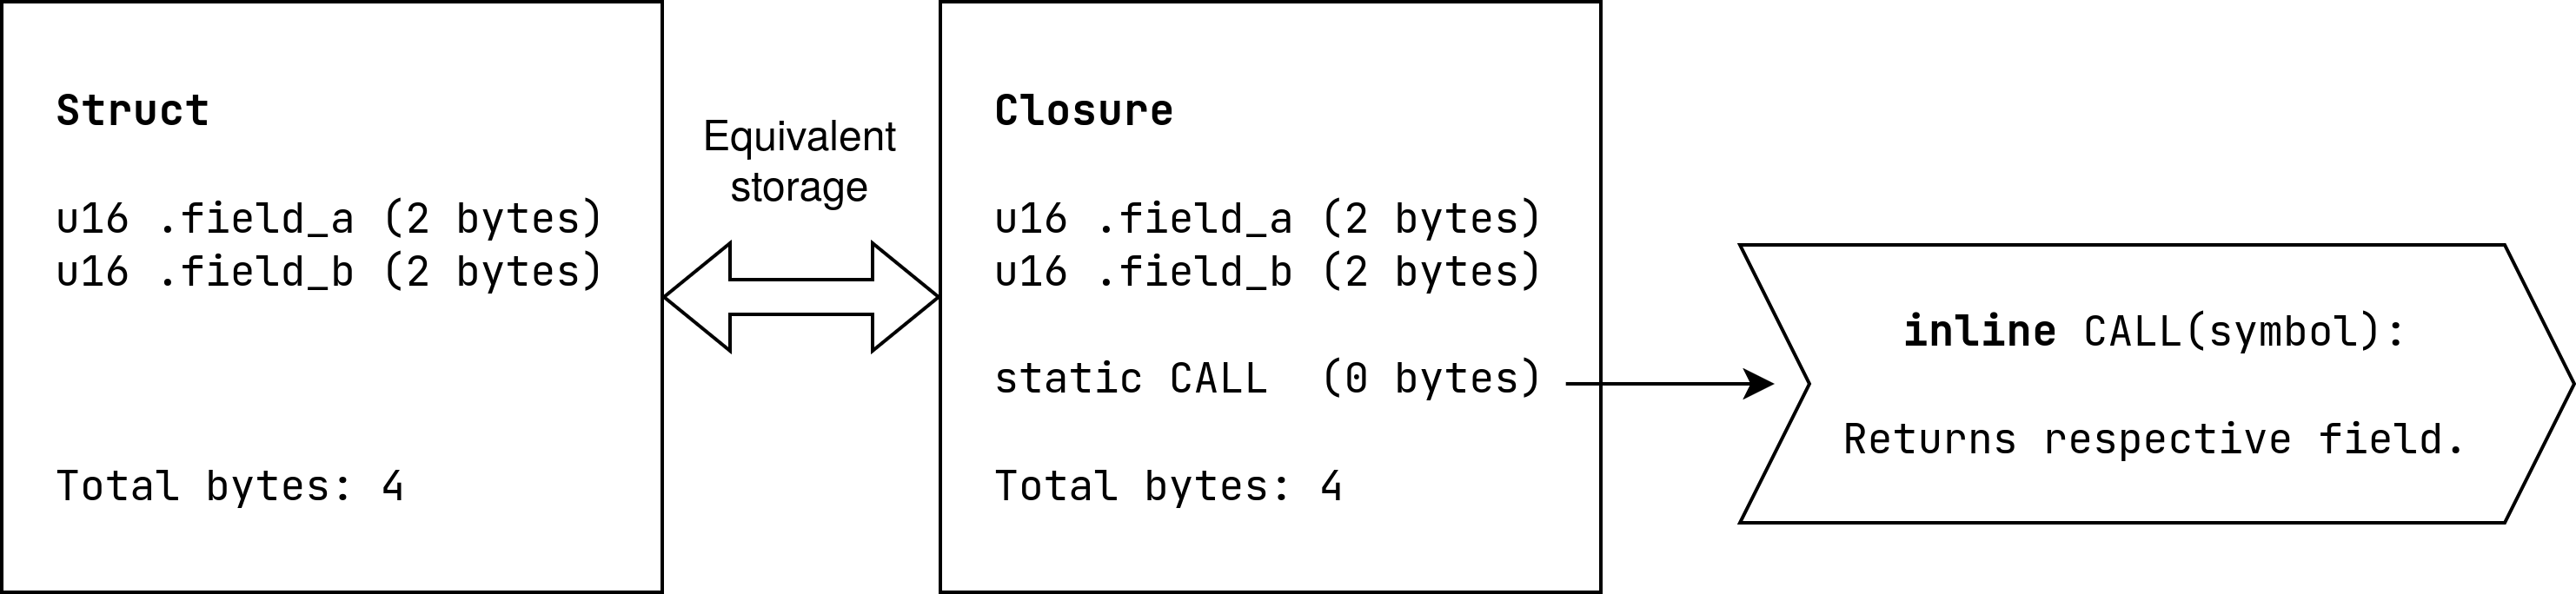
\includegraphics[width=0.9\textwidth]{diagrams/diagram01.png}
  \caption{This diagram showcases the equivalent data representation between a traditional struct (left) and a field extraction closure (right).}
  \label{fig:closurestuff}
\end{figure}

In the same vein, tuples are implemented as syntactic sugar for maps, where positional syntax is translated into numeric symbol input. One notable outcome of this decision is that there is no concept of multiple function parameters; instead, there is a single parameter which reuses the existing tuple syntax to achieve multiple parameters. It's maps all the way down.

Next, maps and enums are unified via a so-called Map-Enum Equivalence rule: Recall Rust-like enums (tagged unions) where a symbol (:foo\_bar) is associated with some data (:foo\_bar("hello")). A syntactical ambiguirty arises. Writing map:foo\_bar("hello") may be interpreted as first calling the map with a symbol (an enum without data) and then calling the resulting map with ("hello"). It may also be interpreted as calling the map with the fully populated enum (:foo\_bar("hello")). The solution is to unify these two approaches, by demanding that all maps obey map-enum equivalence, that is, that calling a map with a symbol and then another map is equivalent to calling the map with the fully populated enum. This bears partial resemblance with currying: Populated enums can now be understood as pre-curried symbols instead of an entirely distinct concept.

In summary, the vast majority of code written by the programmer now comes from maps and symbols!

\subsection{Body-Map Unification}



\subsection{Type-Value Unification}

Old-fashioned languages treat types and values as entirely distinct. In the traditional sense, a type offers two functions:

\begin{enumerate}
\item It details the runtime representation of the data, i.e. the possible runtime values that may be encoded and how many bits of data are needed.
\item It provides a constraint to the programmer themself if they later modify the code, preventing the programmer from using values that the code is not built for.
\end{enumerate}

It turns out that it may be appropriate for these two intents to diverge. This results in two separate notions of a type:

\begin{itemize}
\item \textbf{Logical Type:} A set of allowable values. A constraint of what theoretical values are permissible, i.e. subject the programmer's intended business logic.
\item \textbf{Encoding Type:} A bijection between a set of values and a set of bit patterns. This allows logical types to be designed and abstracted independent of the encoding used.
\end{itemize}

To achieve this distinction, the syntax for logical types and values are unified by treating everything as a constraint. A value is just a singleton constraint, i.e. one possible value. Types are then merged using a binary reduction algorithm such that the final type meets all constraints. Then, an appropriate type encoding is determined that works in harmony with the logical type.

With this in mind, there is no syntactic differentation between types and values, and there is no syntax to give a variable a type. For instance, as illustrated in \autoref{fig:typevals}, we can assign a variable to a type, a value, or both. Semantically, however, the compiler will bail if it realizes there is no single runtime representation available.

\begin{figure}[h]
  \centering
  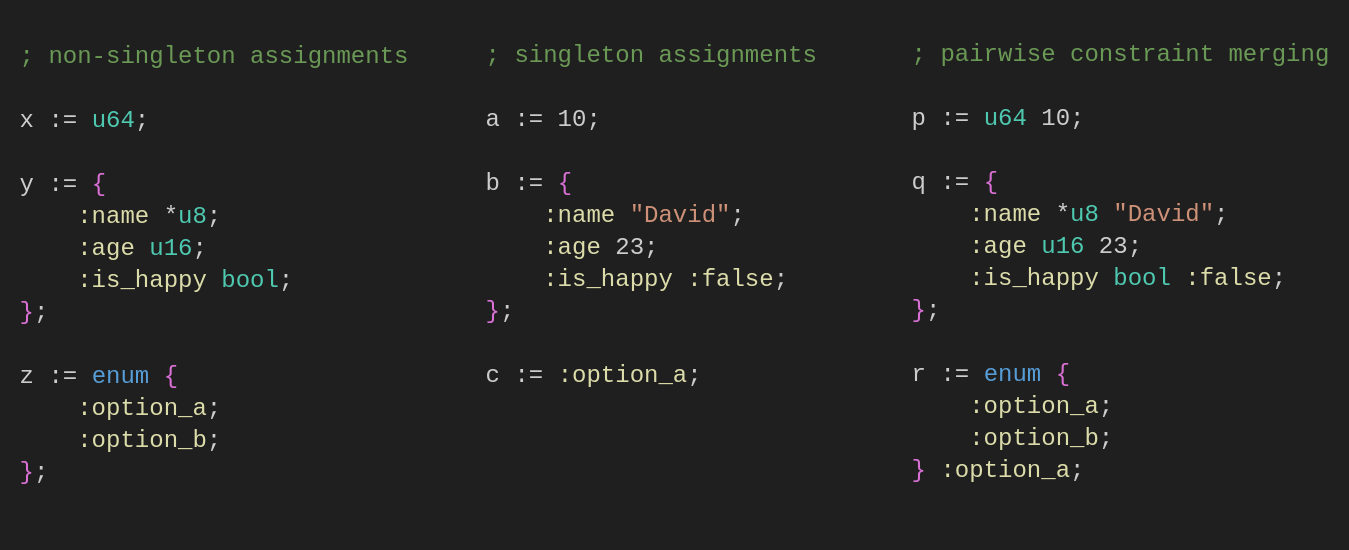
\includegraphics[width=\textwidth]{diagrams/codeblock01.png}
  \caption{How variables can be assigned to a non-singleton type, a singleton type (value), or a pairwise merging of two types.}
  \label{fig:typevals}
\end{figure}


\subsection{Additional benefit of inlining: interacting with existing languages without indirection.}

\subsection{Associativity}

In most programming languages, addition and subtraction are treated as unary operations in an additive batch, whereras operations like multiplication and division are instead treated as binary operations in a multiplicative tree. However, it turns out that any associative operation (such as multiplication) can be written in the former form, where operations in the same family (such as division) control the unary effect via an operator that prefixes the operand. As such, a consistent syntax was employed in this language, allowing both the unary and binary approach for all associative operations and their respective intra-family operations. This includes the following families:

\begin{itemize}
  \item Addition and subtraction (like existing languages);
  \item Multiplication and division;
  \item Logical AND;
  \item Logical OR;
\end{itemize}

The syntax was designed to follow the crystal/pistol pattern, some terminology devised to mean the following:

\begin{itemize}
  \item Crystal: A unary batch of operator/operand pairs (an extension of how existing languages handle addition and subtraction).
  \item Pistol: A binary tree of operations (like how existing languages handle multiplication and division).
\end{itemize}

% For precedence reasons, we have eight separate rules: OR crystal -> OR pistol -> AND crystal -> 
% AND pistol -> additive crystal -> additive pistol -> multiplicative crystal -> multiplicative pistol, with each embedding the next in the hierarchy. Those further to the right of the chain enjoy higher precedence.

More details on this pattern can be gathered from my article on \textbf{\href{https://medium.com/@davidcallanan/rethinking-operation-order-the-illusion-of-ambiguity-and-the-introduction-of-bound-pairs-ceef5242a941}{boundly associative operations}}, my article on \textbf{\href{https://medium.com/@davidcallanan/making-complicated-if-statements-cleaner-61bd1e2afeb8}{making complicated if statements cleaner}}, and my YouTube video on \textbf{\href{https://www.youtube.com/watch?v=C5VEKAc0quk}{rethinking operation order}}.

\begin{figure}[h]
  \centering
  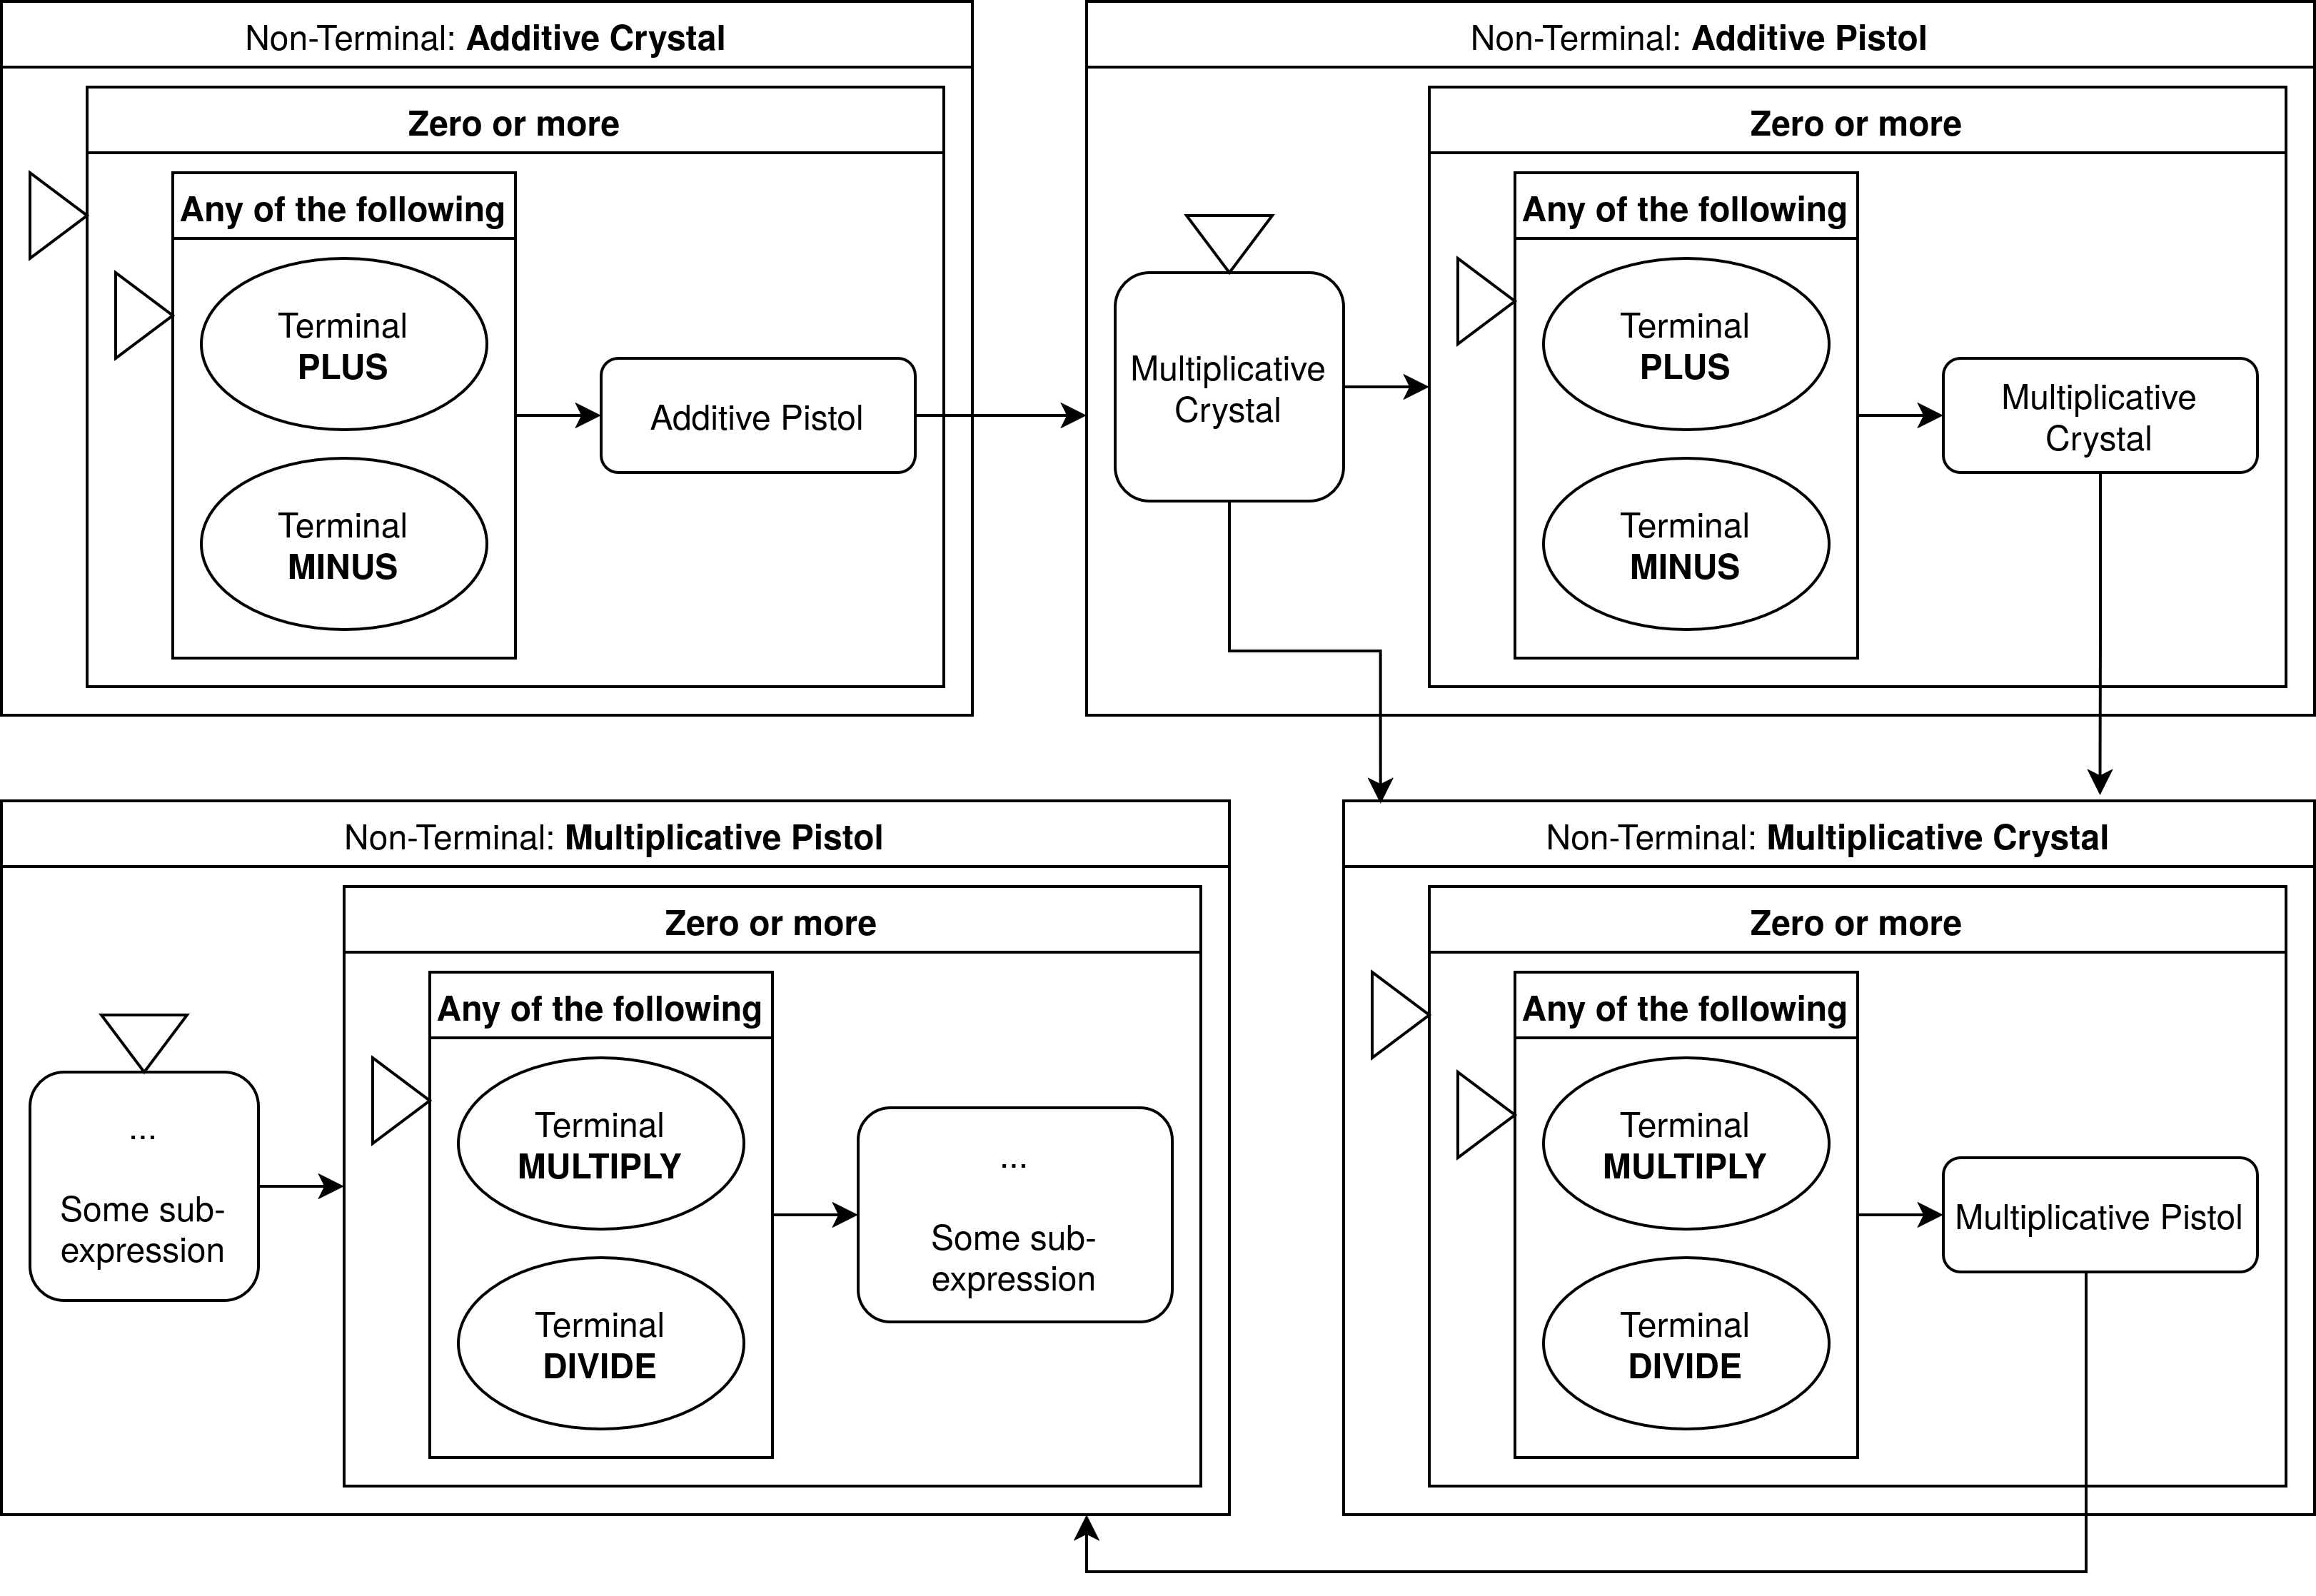
\includegraphics[width=\textwidth]{diagrams/diagram03.png}
  \caption{A simplified extract of some of the associativity and precedence rules for numerical expressions.}
  \label{fig:associativity}
\end{figure}


\subsection{Module Resolution}

Some (debatably legacy) approaches to module resolution are:

\begin{itemize}
\item Use the filesystem alongside symlink functionality to ensure access to the intended modules. This is effective for source code because a single build of a project does not need to switch between versions of source code (if some source code \textit{might} be used, it is \textit{always} included). While multiple instances of source code may be simultaneously deployed, the typing information is fixed. However, many developers consider using the filesystem to be a lot of hassle. Instead, this language takes the stance that if a built-in feature that all developers use (a filesystem) can handle module resolution for types and source code, then why re-invent the wheel. Thus, Essence C promotes the symlink approach for this purpose. This has two consequnences:
\begin{enumerate}
  \item Language-level Ownership: A module takes ownership of type dependencies. While a module may elect to use an external package management solution, symlinks, etc. to resolve the interfaces, by the time the dependencies reach the compiler, the compiler treats the interface as under the ownership of that module. This is favourable to those who follow the dependency inversion principle, but may feel foreign to those who delegate type ownership to external systems.
  \item Monorepos or ``Physical'' Ownership: Those who like to use monorepos or like to own their dependencies physically (that is, not just within the language, but as a non-functional business rule), will have no trouble baking copies of dependencies into their repo. This is a huge reason why many developers (including myself) switched over to the ``pnpm'' package manager for JavaScript projects.
\end{enumerate}
\item Paths: Compare the common use of paths to the Plan 9 operating system. Using paths is arguably messy as it is easy to pollute the global namespace.
\end{itemize}

One must distinguish instance resolution, source code resolution, and type resolution.

As Essence C wants serious static analysis of modules, passing instances is the only solution for the instance part. Spaghetti is avoided by using the factory approach as detailed in the module system.

However, the language takes a balanced approach when it comes to soruce code and type resolution, allowing you to use internal languages features to control the propogatoin of such dependencies. This allows a library to put the burden of populatoin on the user of the library. While this transfers a certain burden of ownership, is unlocks a flexibility that allows developers to not be inmpacted by personal resolution preferences of developers. This is a trade-off that requires further contemplation.

\subsection{Constant By Default}

\subsection{No Standard Library}

With kernel development as the primary target audience for this language, the language should be freestanding and not have any external dependencies. In kernel development, it does not make sense to have built-in functions for most features, as the kernel developer is expected to implement all features themselves (printing, keyboard input, memory allocation, etc.) by communicating directly with the hardware using assembly instructions. Thus, the language only externs one function, ``puts'' , for logging purposes. This function is easy enough to implement early on in kernel development, but the developer can also choose to use a no-op and avoid logging, if they so please.

Rather than a standard library, first class integration with LLVM IR and the C ABI was implemented. This means the code can interact with any code written outside the language, preventing the need for the developer to migrate existing code to Essence C.

\section{Implementation}

\subsection{Build Environment}

Early on in development, I was adamment to ensure a fully reproducible build environment. All building is done using the terminal, so that the build process is independent from the editor used. The JavaScript portion of the project uses \textit{Node.js} and \textit{pnpm}, which are easy to install on different operating systems. Build scripts are then organized into \textit{package.json} files. However, the C++ portion, consisting of a suite of tools (\textit{clang}, \textit{make}, \textit{llvm}, etc.), is more difficult to set up consistently. The build scripts for this portion are organized using a Makefile, and the development environment itself is prepared using a Dockerfile. Some developer scripts were implemented in Bash to orchestrate the overall process between the JavaScript and C++ portions, the Docker layer, and the developer's own environment. The choice to use Bash means the developer must either use a Linux environment or a WSL environment if using Windows. A docker-in-docker strategy could theoretically have been used instead, requiring minimal platform-specific scripts, but this complexity was avoided. MacOS users may suffer as a result. Additionally, I recently switched to NixOS on my own system, and its philosophy was applicable here. NixOS allows you to write description-based software setups, which can act as reproducible development enviornments. Thus I set up a repository-level Nix script for those on NixOS who want to fast-track setting up their development environment. This makes both the build layer and host interaction layer highly reproducible.

\subsection{Parsing}

Prior to this project I had already developed a simple parsing library in JavaScript, which allows for:

\begin{enumerate}
	\item Parsing terminal rules using regular expressions.
	\item Forming non-terminal rules by combining other rules in the following ways (sufficient to develop any complex grammar): \begin{itemize}
	\item ``or'': making a rule optional
	\item ``join'': sequencing rules
	\item ``multi'': repeating rules zero or more times
	\item ``opt'': making a rule optional
	\item ``lookAhead'': peeking ahead to prevent ambiguity (seldom used)
	\end{itemize}
	\item Map parsed data to custom structures using the ``mapData'' function.
\end{enumerate}

Essence C was then parsed by handcrafting hundreds of parse rules using this library.

\begin{figure}[h]
  \centering
  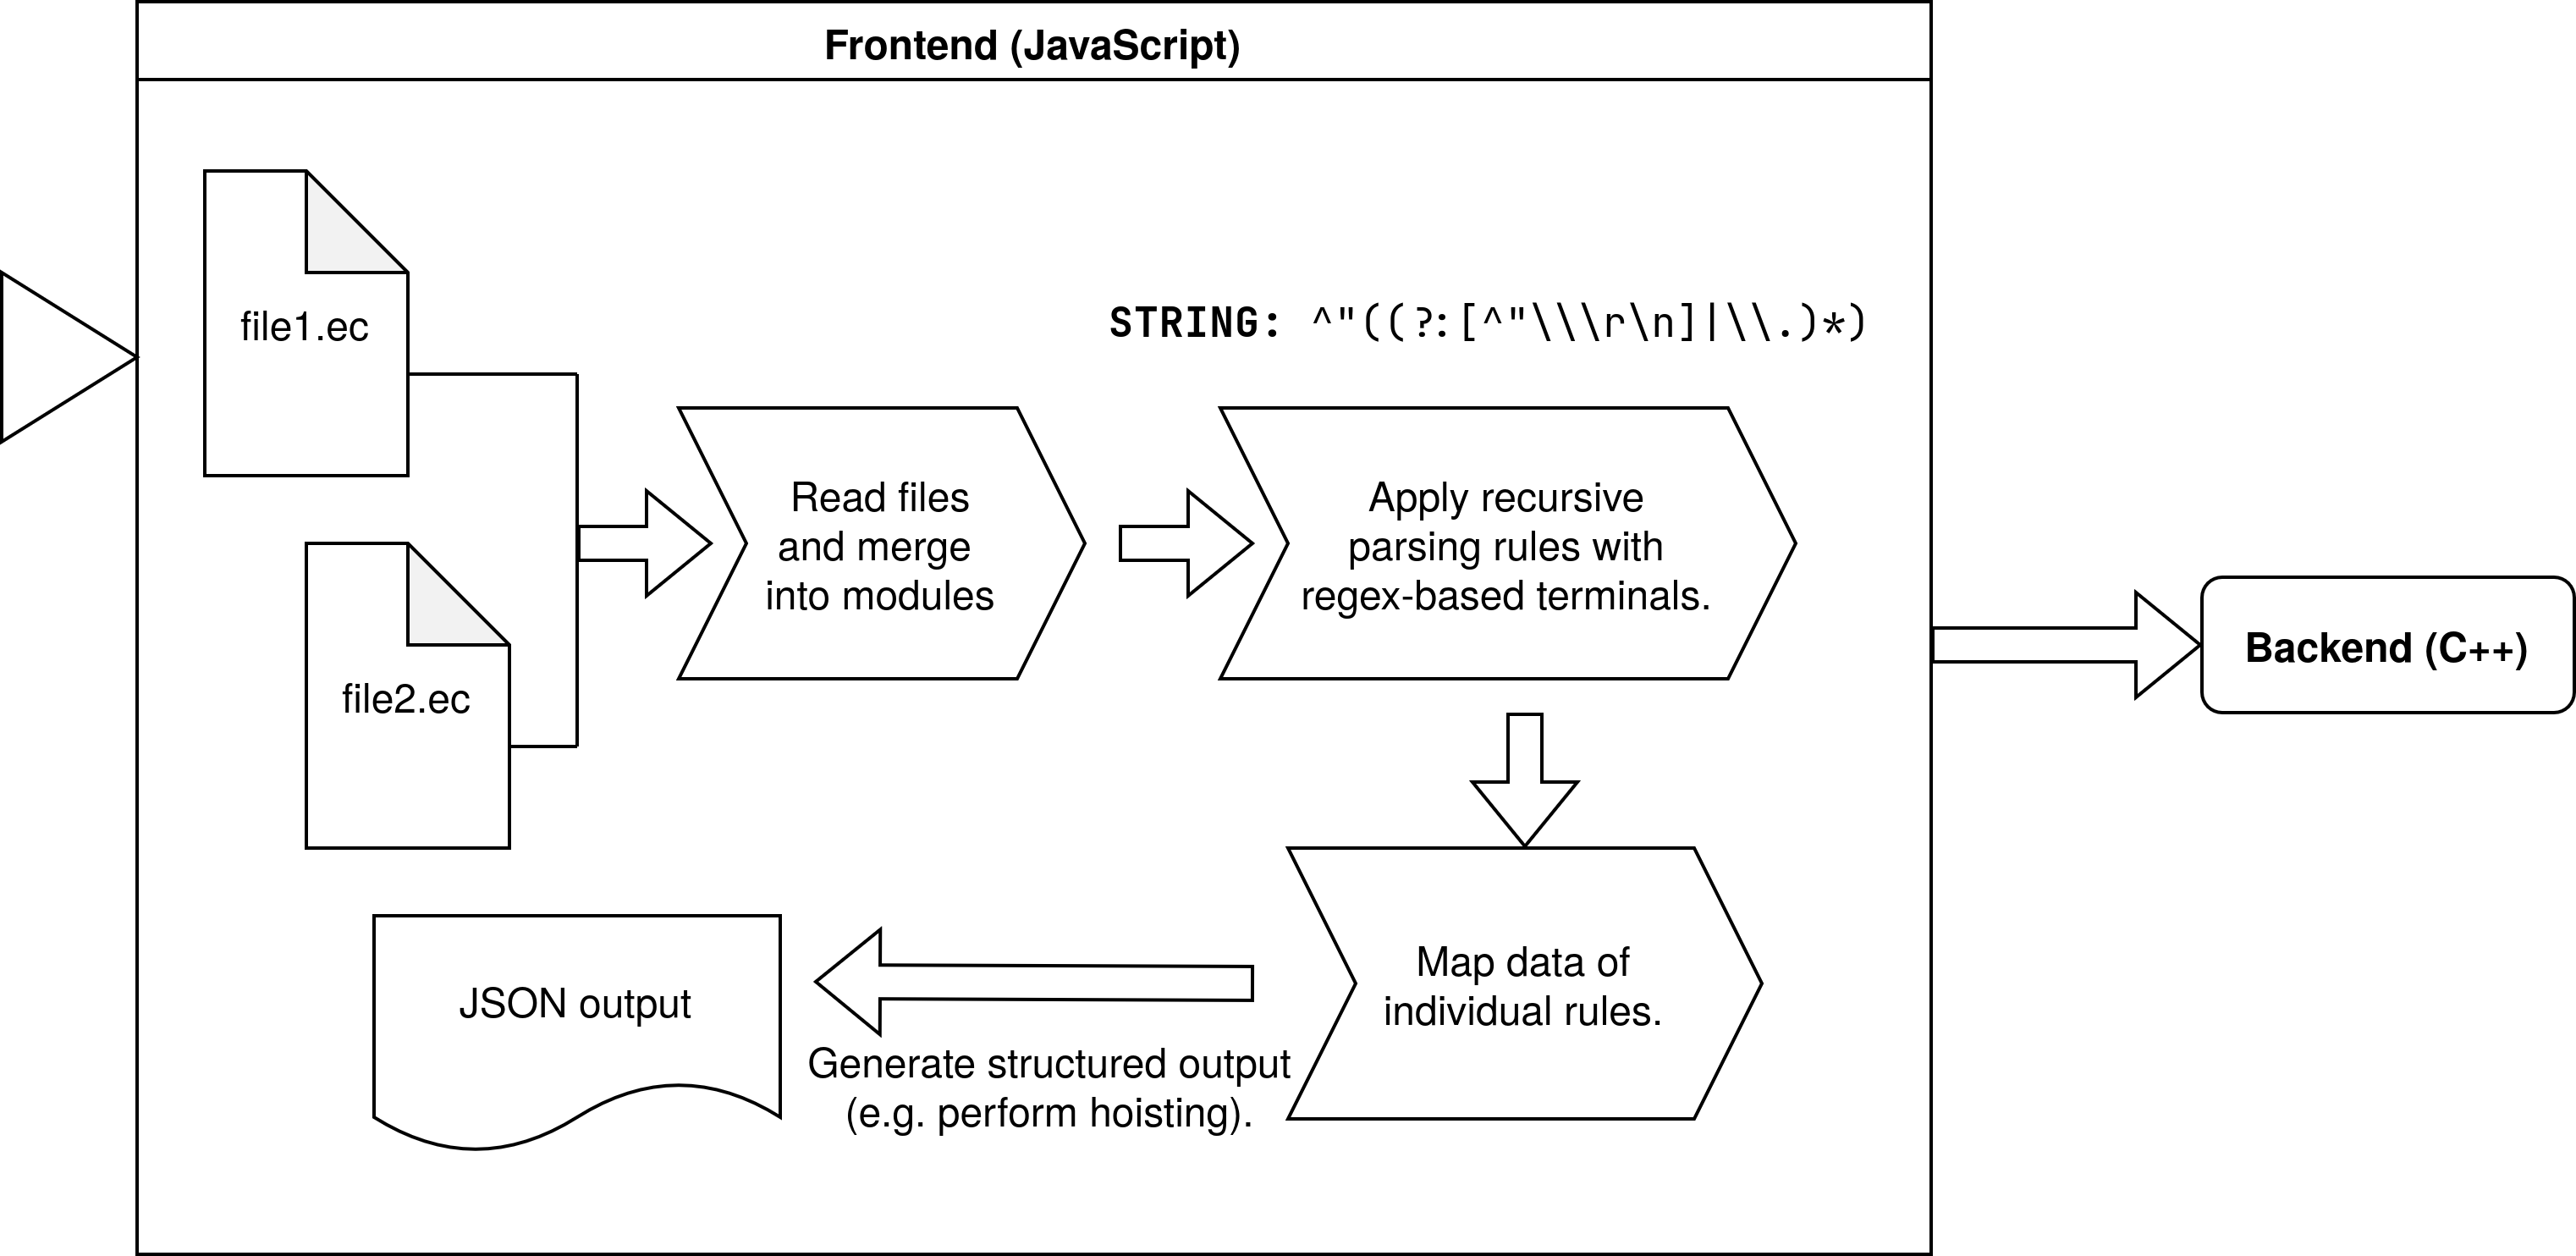
\includegraphics[width=\textwidth]{diagrams/diagram02.png}
  \caption{High-Level Frontend Architecture}
\end{figure}


\subsection{Parser Trace Explorer}

Parsing issues were frequently encountered during the development cycle, and manual debugging became infeasible as complexity increased. Hence, a \textit{Parser Trace Explorer} was developed, consisting of a JSON trace logger in the compiler frontend, and a separate web-app tool for exploring these logs. A simple SolidStart + Tanstack Router tech stack was selected for this tool due to existing familiarity with this stack, and because of the straightforward requirements of the tool.

Since parsers try a vast number of rules and are inherently recursive, the logs quickly exceed $500,000$ lines for small source files. To deal with this, the logs are structured as a tree, and the user of the tool is expected to navigate this tree by selecting the precise rule attempts that the parser is supposed to succeed on, thus hiding irrelevant attempts. A dedicated lexer, in hindsight, would have reduced the exponential growth of the logs, but might not have easily parsed some of the unique language features (such as semicolons acting as both terminators and comments).

\begin{figure}[h]
  \centering
  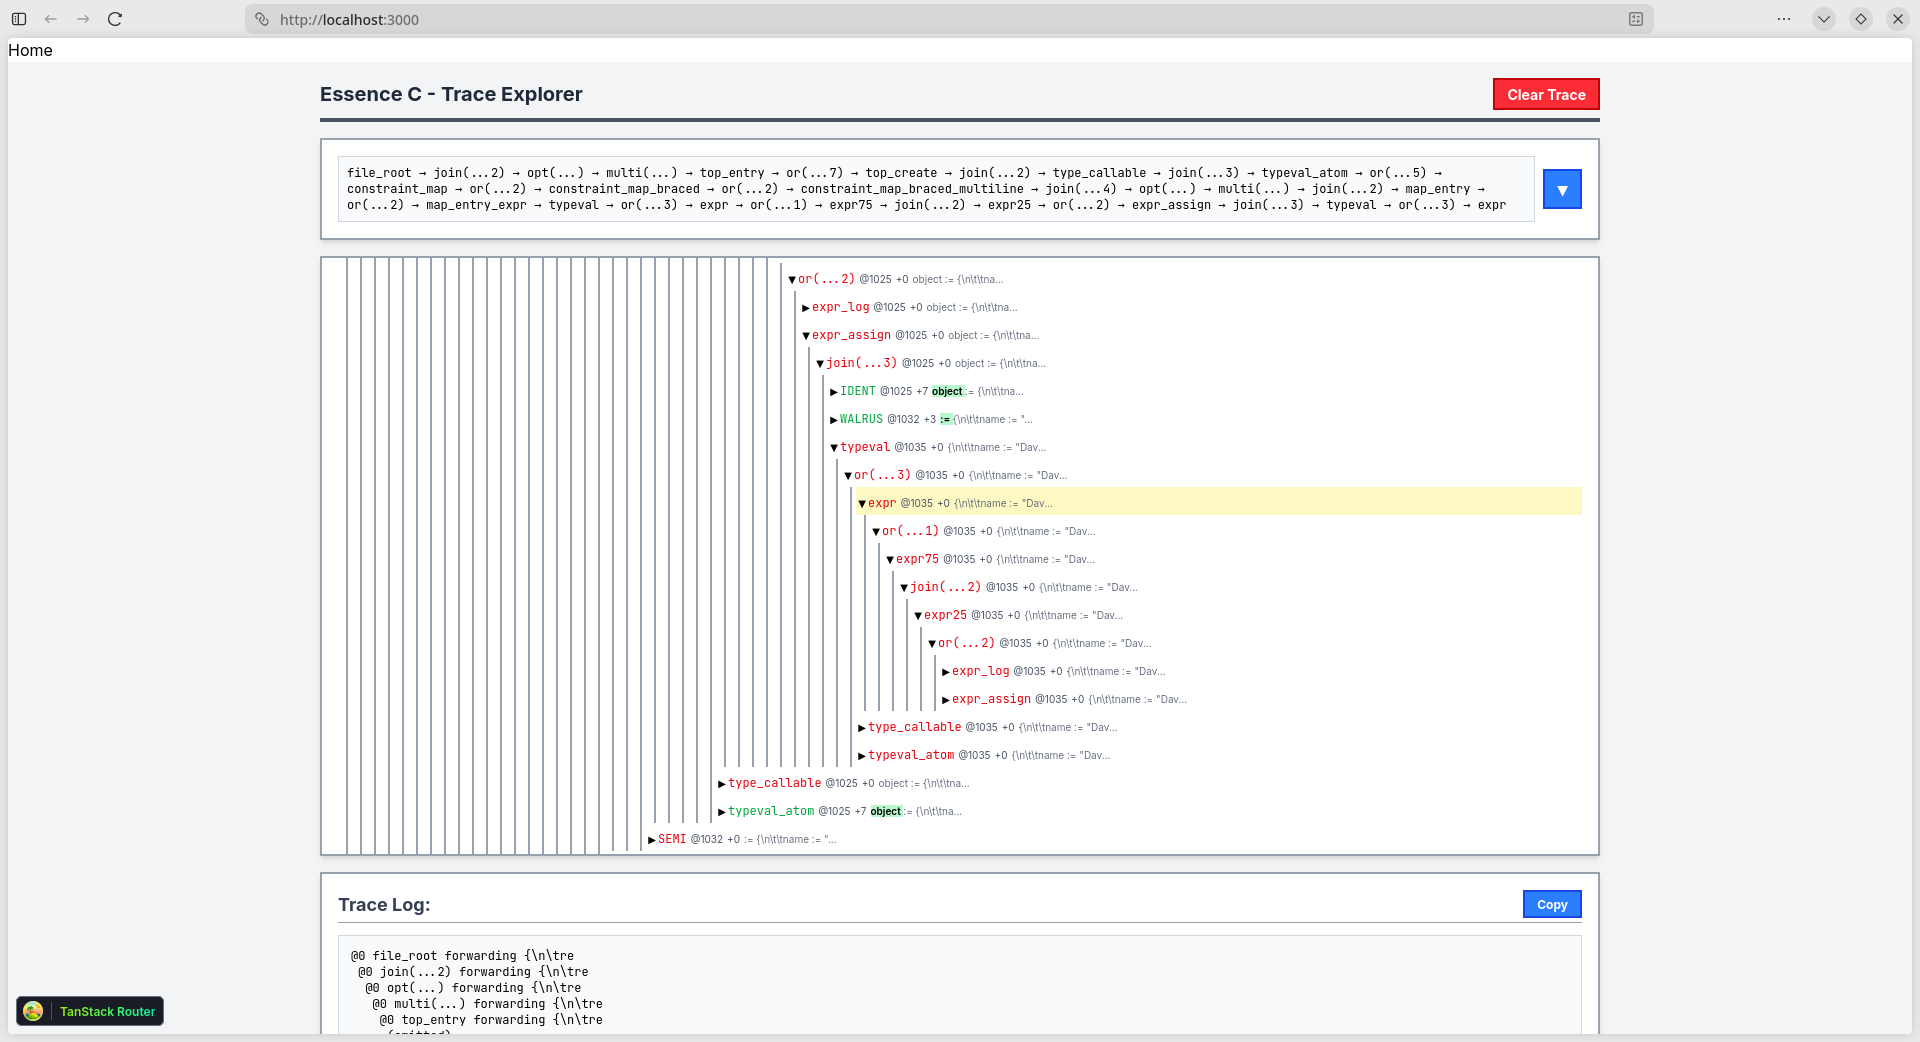
\includegraphics[width=\textwidth]{screenshots2/trace_explorer_00.png}
  \caption{Parser Trace Explorer}
\end{figure}


\subsection{Defensive Programming}

As Essence C is designed with strict semantics, the backend has no need to recover from illegal states. As such, defensive programming is used, where the program is crashed with a useful error message whenever an invariant is violated. Such errors could originate from semantic violations in the user's code, or due to subtle bugs in the compiler itself; either way, the issues can be traced effectively. Naturally, not all subtleties can be pre-envisioned, so this was done on a best-effort basis to avoid compromising development speed.


\subsection{Mutability Support}

LLVM IR is in SSA form, where registers are immutable. One cannot reuse a register, and must instead create a new register for every mutation. Then, one takes advantage of the phi instruction to pick which register is the correct one at runtime. However, the alloca (stack allocation) model operates under the familiar mindset of mutability, as it works with raw memory addresses. Conveniently, it was observed that the standard mem2reg optimization pass does a fantastic job at converting stack allocations into SSA registers where legal, bypassing the tough development of a custom SSA mutability mechanism. Thus, variables are entirely implemented using stack allocations. This saved an estimated week of development time.

\subsection{Debugging Primitives}

While the primary mechanism of performing external communication is to link with external code via the C ABI (which may be LLVM IR), debugging functionality is often preferable within the language directly in case there are issues with the interoperability layer proper. Thus, two basic logging functions were implemented, ``log'' and ``log\_d''. The former takes a null-terminated ascii string and prints this output in an implementation-specific manner. The latter takes an arbitrarily-sized value (like an integer or a byte array) and prints its raw binary representation (in 64-bit chunks), including both its hex representation, ascii representation, and decimal representation. The implementation of this functionality was chosen to be implementation-specific. In the prototype implementation, the external ``puts'' function was selected to implement this functionality, available in many environments. In case the environment does not support it, a dummy no-op implementation can be defined, effectively dropping any logs.

\subsection{Bit-width Analysis}

Determining the maximum bits needed to hold an integer is an important optimization. While LLVM may be able to detect certain constraints about numbers, much of the compiler information is lost at this point that a modern programming language might be interested in tracking. For example, software verification languages may keep track of exact min and max values for an integer type, which is tracked extensively as the type system navigates the codebase. For non-integer types, an optimal type system implementation might allow the user to use formal logic to keep track of the theoretically-smallest set of runtime possibilities (a provably accurate picture of the possible values that can be assigned at runtime, with no wasted space).

Only simple bit-tracking is performed in the prototype compiler. When a hardcoded integer constant is used, the number of bits is trivially calculated using the logarithm. Addition was more tricky to implement -- one must recursively track the bits needed to hold an arbitrary sum of other integers. The first attempt of taking the maximum of the operand bits and adding one (to account for a potential carry) was insufficient for more than two operands. While an additional carry bit could be added for each additional operand, this estimate would be too conservative. The correct solution was to sum the maximum value each operand could take on (interpreted as data to avoid to intricacies of signed integers), and then take the logarithm of this sum. This can achieved easily in languages that support arbitrarily sized integers out-of-the-box. However, it was easier to implement an approximate solution in C++ by using the double data type, with the final result rounded up. While this sounds bizarre and inaccurate at first glance, recall that floats are internally implemented using an exponent and mantissa. Thus, it is very similar to running the numbers through a logarithmic transformation, which would yield the final result directly. Furthermore, an epsilon value was included to deal with precision errors, favouring a more conservative bit estimate. It was not proven whether this overall approach is mathematically sound up to a particular bit count, but it can always be substituted if the need arises.

\subsection{Underlying Type Tracking}

\subsection{Singletonish Optimization}

A custom "singletonish" optimization was implemented that concerns itself with both the module optimizatoin goal (detecting something to be static) and the acknowledgement of the benefits of singleton types (by treating lonely values as singleton types). It also is meets the demands of the map enum equivalence, central to the design of the module system, as it allows different aspects of maps which are inherently static (e.g. the functional nature of maps) to be optimized to a form that behaves like traditional programming languages. This means the map-enum equivalence is not just theoretical, but acutually works.

\subsection{Static Instance Analysis}

\chapter{Evaluation (930)}

\section{Manual Snapshot Testing}

Throughout the development cycle, manual testing was conducted by compiling sample source files and inspecting the terminal output after running the final executable. This mirrors the snapshot testing philosophy commonly implemented in web-development projects (although accomplished in a less automated fashion here), where input/output consistency is checked before each commit to source control. Down the road, this strategy could be extended to a full test suite that prevents all sorts of regressions. One could take this a step further by checking consistency in the compiled LLVM IR code itself, but this is typically only done when a language reaches a pivotal level of maturity; the compiler is in too much flux at this point for this technique to have any merit.

Much of the snapshot testing was performed using the language's data logging facility which prints the hexidecimal, ascii, and decimal values of arbitrarily-sized binary sequences. This allows straightforward investigation of any runtime values, whether that be integers, floats, pointers, strings, enums, and so on.

% \section{User Acceptance Testing}

% Four students from Maynooth University were tasked with implementing a program in the language. Each student was asked to provide positive and negative feedback of the solution.

% The users were given the following code with no explanation, but were allowed to ask me questions.


% \renewcommand{\arraystretch}{1.4}
% \begin{longtable}{|>{\raggedright\arraybackslash}p{5.5cm}|>{\raggedright\arraybackslash}p{\dimexpr\textwidth-5.5cm-4\tabcolsep-2\arrayrulewidth\relax}|}
% \caption{Feedback survey}\label{tab:uat} \\
% \hline
% \textbf{Question} & \textbf{Answer} \\
% \hline
% \endfirsthead
% \hline
% \textbf{Question} & \textbf{Answer} \\
% \hline
% \endhead
% \hline
% \endfoot
% \multicolumn{2}{|l|}{\textbf{Student A}} \\
% \hline
% What is the sample program doing? & [Answer] \\
% \hline
% What semantic or syntactic element of the sample program strikes you the most, and why? & [Answer] \\
% \hline
% Implement a program that does blah. Provide one point of positive feedback about the language. & [Answer] \\
% \hline
% Provide one harsh criticism about the language. & [Answer] \\
% \hline
% \multicolumn{2}{|l|}{\textbf{Student B}} \\
% \hline
% What is the sample program doing? & [Answer] \\
% \hline
% What semantic or syntactic element of the sample program strikes you the most, and why? & [Answer] \\
% \hline
% Implement a program that does blah. Provide one point of positive feedback about the language. & [Answer] \\
% \hline
% Provide one harsh criticism about the language. & [Answer] \\
% \hline
% \multicolumn{2}{|l|}{\textbf{Student C}} \\
% \hline
% What is the sample program doing? & [Answer] \\
% \hline
% What semantic or syntactic element of the sample program strikes you the most, and why? & [Answer] \\
% \hline
% Implement a program that does blah. Provide one point of positive feedback about the language. & [Answer] \\
% \hline
% Provide one harsh criticism about the language. & [Answer] \\
% \hline
% \multicolumn{2}{|l|}{\textbf{Student D}} \\
% \hline
% What is the sample program doing? & [Answer] \\
% \hline
% What semantic or syntactic element of the sample program strikes you the most, and why? & [Answer] \\
% \hline
% Implement a program that does blah. Provide one point of positive feedback about the language. & [Answer] \\
% \hline
% Provide one harsh criticism about the language. & [Answer] \\
% \hline
% \end{longtable}


\section{GenAI Comprehension Testing}

With kernel development as the core case study for this project, the ability for LLMs to understand \textit{Essence C} was assessed by tasking an LLM agent with porting a portion of a previously-written PoC operating system kernel from \textit{C} to \textit{Essence C}. The original kernel was developed as part of my \href{https://www.youtube.com/watch?v=FkrpUaGThTQ&t=2s}{YouTube tutorial series}, and its latest source code is housed in a \href{https://github.com/davidcallanan/os-series}{separate repository here}. The ported version is included in this project's repository. It includes C, Essence C, NASM Assembly, and LLVM IR Assembly code living in unison, with build options to substitute different implementations of the source code.

The LLM agent was first asked to generate documentation for the language, and subsequently to port some benchmarking code into \textit{Essence C}. The prompts and results can be found in Appendix X.

Some slight guidance had to be given to the agent, but for the most part, it was well equipped to handle the task. This is promising as it shows that the agent took no issue with comprehending the unique language syntax and corresponding semantics (specifically, the notions of maps, symbols and modules). Note, however, that the build steps were all implemented manually as this is outside the scope of language comprehension.

\section{Benchmarking}

To kill two birds with one stone, benchmarking was performed on the actual kernel ported by the AI agent, instead of creating artificial benchmarks. Four procedures were benchmarked across three different implementations.

Procedures:

\begin{table}[h]
\centering
\begin{tabular}{|l|p{12cm}|}
\hline
\textbf{Benchmark} & \textbf{Description} \\
\hline
PIT & Accesses the Programmable Interval Timer counter as frequently as possible via the x86 port I/O interface. This is a counter exposed by the x86 hardware that decreases rapidly over time. \\
\hline
RTC & Accesses the Real-Time Clock as frequently as possible via the same interface. The irony is that the RTC is furthermore used in all benchmarks to calculate the actual operations per second. \\
\hline
I/O Wait & Triggers the ``0x80'' hardware request as frequently as possible via the same interface, a legacy no-op instruction that gives the hardware a moment to breathe. \\
\hline
VGA Cursor & Updates the VGA text-mode cursor position as frequently as possible via the same interface. This cursor position controls where text would be printed on the screen when using the basic VGA text interface exposed by the hardware. \\
\hline
\end{tabular}
\caption{The four kernel procedures that are benchmarked.}
\label{tab:benchmarks}
\end{table}

Implementation Variants:

\begin{table}[h]
\centering
\begin{tabular}{|p{2.25cm}|p{1.5cm}|p{11cm}|}
\hline
\textbf{Language} & \textbf{Mode} & \textbf{Details} \\
\hline
C + NASM Assembly & N/A & Baseline implementation. Compiled with GCC with separate compilation units, with limited link-time optimization available. Instances are passed as pointer arguments, and a vtable is implemented to enable implementation swapping. This reflects a real-world C codebase that is architected to be implementation-agnostic. \\
\hline
Essence C + LLVM IR Assembly & Dynamic & Essence C implementation. Linked with LLVM. Instances are passed as pointer arguments, and the language uses a vtable internally to enable implementation swapping. This reflects how a programmer might architect their codebase to be implementation-agnostic. \\
\hline
Essence C + LLVM IR Assembly & Static & Same as above, but a custom ``alwaysinline'' flag is included, and a custom ``mut'' flag is excluded, signalling to the compiler to attempt to make instances static. The compiler succeeds without requiring the programmer to make any architectural changes to their codebase. (These optimizations could be automated at a later stage without requiring these flags).\\
\hline
\end{tabular}
\caption{The three implementation variants tested for each benchmark.}
\label{tab:implementations}
\end{table}

\section{Validation}

\chapter{Conclusion (930)}

\section{Overall Assessment}

Given the time constraints for this project, the evaluation only scratched the surface. One would want to spend the following time:

\begin{itemize}
  \item 200 more hours on this.
  \item 200 more hours on that.
\end{itemize}

Build times consistently exceeding 90 seconds. This is dreadful when debugging and making small tweaks. A professional C++ developer would likely have experience optimizing the build process.

\section{Contribution to state-of-the-art}

- inlining
- built in language constructs to avoid likes of kernel static\_call
- continuum of dispatch, not just static vs dynamic, but by merging the notion of class instances (and fusing classes and modules), if we detect multiple instances we can switch to an even more dynamic dispatch mechanism.
- more efficient inter-language interoperability

\section{Limitations}

\begin{itemize}
  \item The prototype compiler does not yet support cross-compilation. This means a Windows executable cannot be built from within a Linux build environment, or vice versa. Thus, everything had to be kept to Linux/WSL for now.
  \item The parser does not produce helpful error messages. Thus, one must either use a pair of eyes to identify syntax errors, or use the bulky \textit{Parser Trace Explorer} to investigate more significant issues.
  \item With more time, the entire kernel could have been migrated from \textit{GCC} to \textit{Clang}. This would have offered more realistic benchmarks given \textit{Clang}'s superior link-time optimizations over \textit{GCC}. Nonetheless, the effort of such a migration reminds us of the struggles developers face when writing software in C today -- struggles that might be less prevalent in a language like \text{Essence C} that treats LLVM IR as a first-class citizen.
  
\end{itemize}

  \section{Future Work}
  

\newpage

\printbibliography[title=References]

\appendix

\includepdf[
    pages={1},
    frame, 
    scale=0.6, 
    pagecommand={\thispagestyle{plain}
\chapter{Record of Meetings} \vspace{175mm}}
]{./appendix_meetings.pdf}

\newpage

\chapter{Screenshots}

% \input{appendix_screenshots.tex}

\newpage

\chapter{Source Code}

Included in this appendix is a snapshot of the project repository as of the date of submission of this interim report. The full repository, including the entire git history, is available upon request. Please request access to the private repository located at \href{https://github.com/davidcallanan/mu-fyp}{https://github.com/davidcallanan/mu-fyp}.

Build artifacts and other uninteresting files have been omitted from this appendix. This includes, but is not limited to, all files mentioned inside \lstinline{.gitignore}.

% \input{appendix_source_code.tex}

\newpage

\chapter{LLM Prompts}

% \input{appendix_llm_prompts.tex}

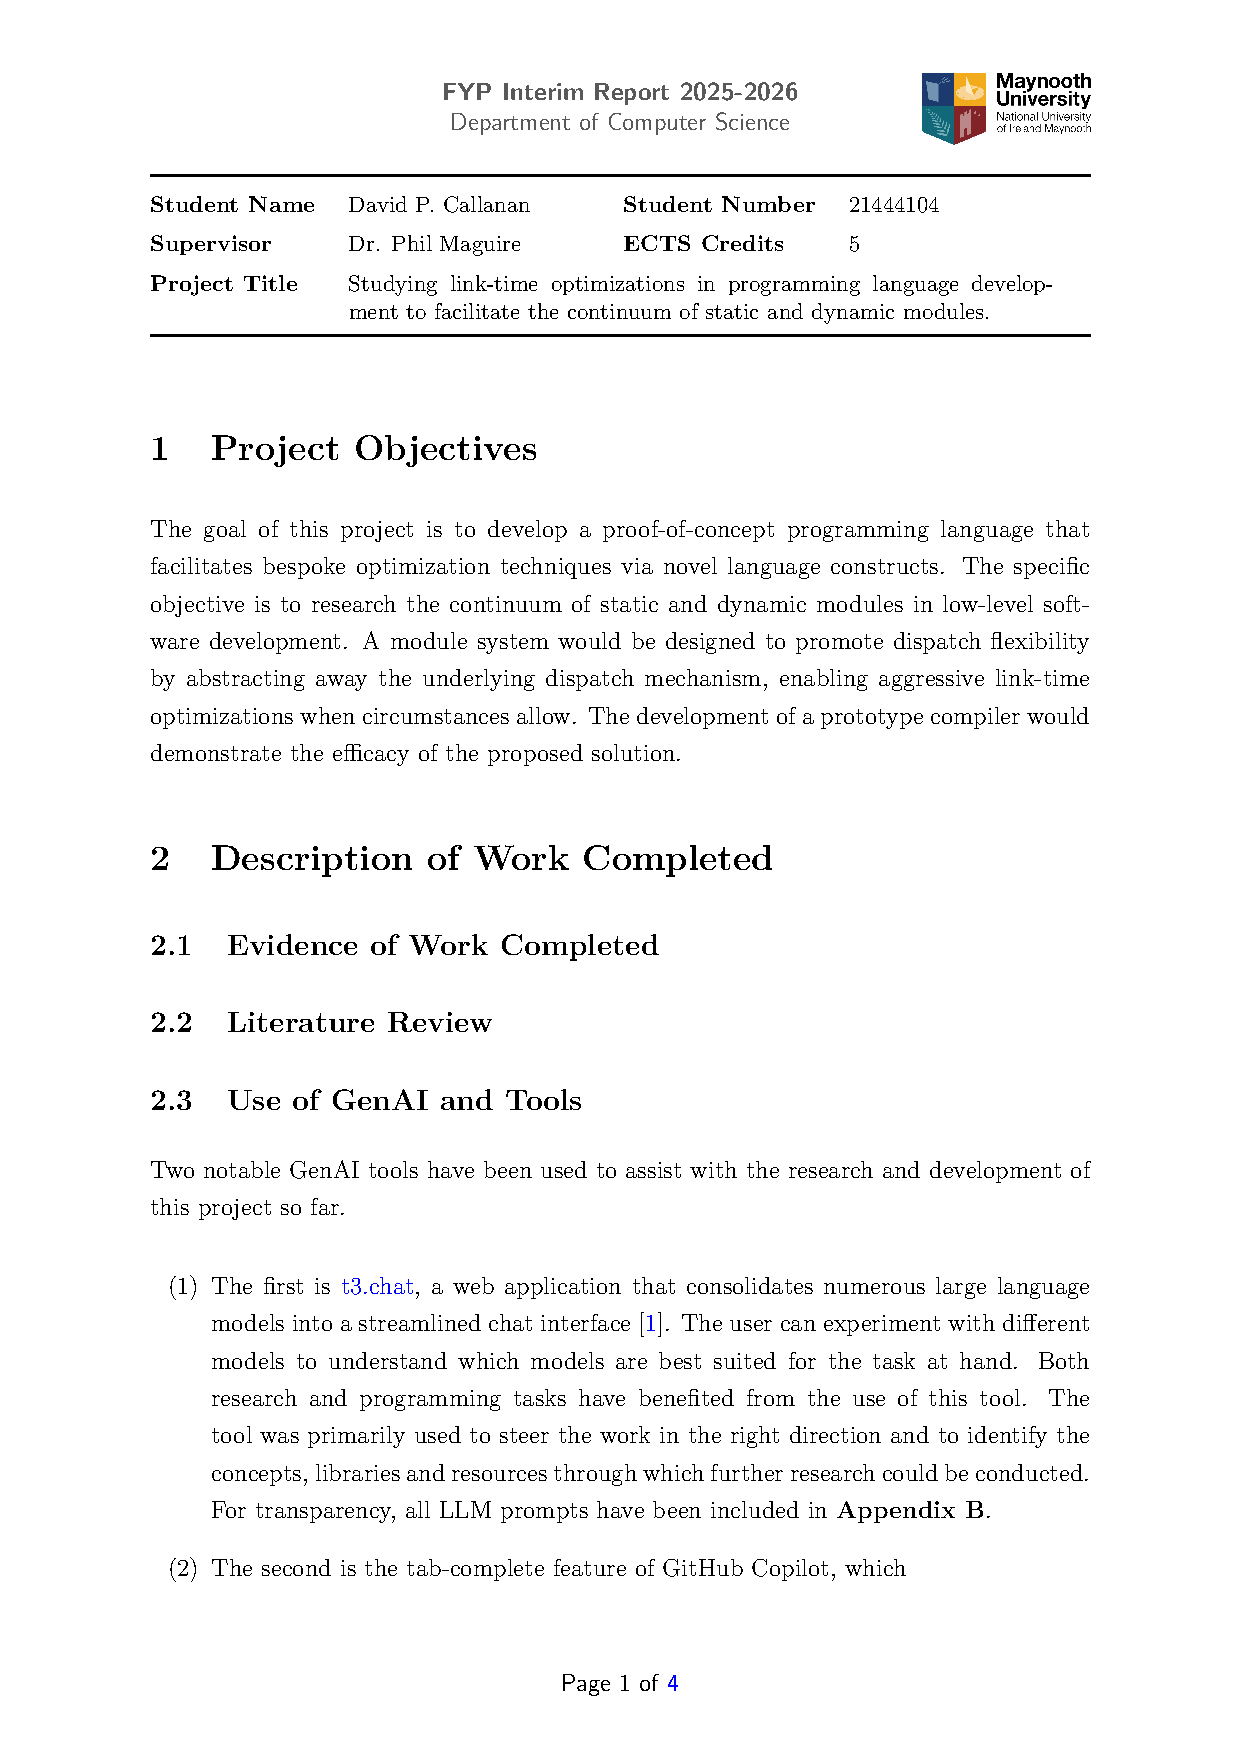
\includepdf[
    pages={1},
    frame, 
    scale=0.65, 
    pagecommand={\thispagestyle{plain}
\chapter{Interim Report}}
]{../2511_interim_report/report.pdf}


\includepdf[
    pages={2-5},
    frame, 
    scale=0.75, 
    pagecommand={\thispagestyle{plain}}
]{../2511_interim_report/report.pdf}

\label{LastPage}
\end{document}
